
\include{./def/yf-formatting}
\include{./def/yf-def}

\usepackage{wasysym}
%\usepackage{times}

\title{}
\author{}
\date{}


\def\A{\mathcal{A}}
%\def\B{\mathcal{B}}
\def\C{\mathcal{C}}
%\def\D{\mathcal{D}}
\def\E{\mathcal{E}}
\def\FF{\EuScript{F}}
\def\G{\mathcal{G}}
\def\GG{\EuScript{G}}
\def\H{\mathcal{H}}
\def\I{\mathcal{I}}
\def\J{\mathcal{J}}
\def\L{\mathcal{L}}
\def\Q{\mathcal{Q}}
\def\S{\mathcal{S}}
\def\T{\mathcal{T}}
\def\V{\mathcal{V}}
%\def\W{\EuScript{W}}
\def\W{\mathscr{W}}
\def\X{\mathcal{X}}
\def\Y{\mathcal{Y}}
\def\Z{\mathcal{Z}}


\def\bad{\mit{bad}}
\def\bigmid {\, \Big\lvert \,}
\def\capacity{\mit{cap}}
\def\clean{\mit{clean}}
\def\con{\mit{con}}
\def\cost{\mit{cost}}
\def\cut{\mit{cut}}
\def\det{\mit{det}}
\def\dis{\textrm{DIS}}
\def\dom{\succ}
%\def\domby{\prec}
\def\dombyeq{\preceq}
\def\domeq{\succeq}
\def\err{\mit{err}}
\def\errate{\mit{err}\textrm{-}\mit{rate}}
\def\good{\mit{good}}
\def\lab{\mit{label}}
\def\loc{\textrm{loc}}
\def\middle{\mit{mid}}
\def\mono{\mathbb{H}_\mit{mon}}
\def\neg{\mit{neg}}
\def\newstar{\circledast}
\def\pos{\mit{pos}}
\def\ran{\mit{ran}}
\def\rest{\mit{rest}}
\def\rpe{\mathrm{RPE}}
\def\siml{\mathit{sim}}
\def\sink{\sqsupset}
\def\src{\sqsubset}
\def\starnum{\mathfrak{s}}
\def\totalcost{\mit{family\textrm{-}cost}}
\def\totalerr{\mit{family\textrm{-}err}}
\def\weight{\mit{weight}}
\def\werr{\mit{w}\textrm{-}\mit{err}}

\def\extraspacing{\vspace{4mm} \noindent}
\def\vgap{\vspace{4mm}}
\def\vslit{\vspace{2mm}}

\begin{document}

\boxminipg{\linewidth}{
    \begin{center}
        \vspace{3mm}
    {\Large
    (CE7456 Lecture Notes 15) Monotone Classification} \\[2mm]
    {\large Yufei Tao}
    \vspace{3mm}
    \end{center}
}

This lecture discusses a problem from active learning named {\em monotone classification}.


\extraspacing {\bf Math Conventions.} For an integer $x \ge 1$, the notation $[x]$ represents the set $\set{1, 2, ..., x}$. Given a predicate $Q$, the notation $\mathbbm{1}_Q$ equals 1 if $Q$ holds or 0 otherwise.

\section{Problem Definition} \label{sec:prob}

The input is a multiset $P$ of $n$ points in $\real^d$ for some integer $d \ge 1$. The multiset may contain repeated points, that is, distinct elements with identical coordinates. Each element $p \in P$ carries a label from $\set{-1, 1}$, which is represented as $\lab(p)$.

\vgap

A {\em classifier} is a function $h: \real^d \rightarrow \set{-1, 1}$. We say that $h$ {{\em correctly classifies}} an element $p \in P$ if $h(p) = \lab(p)$, or {\em misclassifies} $p$, otherwise. The {\em error} of $h$ on $P$ is defined as
\myeqn{
    \err_P(h) &=& \sum_{p \in P} \mathbbm{1}_{h(p) \neq \lab(p)} \label{eqn:err-classifier}
}
that is, the number of elements in $P$ misclassified by $h$. A classifier $h$ is {\em monotone} if $h(p) \ge h(q)$ holds for any two points $p, q \in \real^d$ satisfying $p \dom q$.

\vgap

Define
\myeqn{
    \mono &=& \text{the set of all monotone classifiers} \label{eqn:monoclass} \\
% }
% Set
% \myeqn{
    k^* &=&
    \min_{h \in \mono} \err_P(h). \label{eqn:k-star}
}
We call $k^*$ the {\em optimal monotone error of $P$}. A classifier $h \in \mono$ is {\em $c$-approximate} on $P$ if $\err_P(h) \le c \cdot k^*$ where $c \ge 1$ is the {\em approximation ratio} of $h$.


\vgap

    Figure~\ref{fig:intro-ds} shows a 2D input $P$ where a black (resp., white) point has label 1 (resp., $-1$). Consider the monotone classifier $h$ that maps (i) all the black points to 1 except $p_1$, and (ii) all the white points to $-1$ except $p_{11}$ and $p_{15}$. Thus, $\err_P(h) = 3$. No other monotone classifier has a smaller error on $P$ and, hence, $k^* = 3$. Consider the classifier $h^\pos$ that maps the entire $P$ to $1$. It can be verified that $\err_P(h^\pos) = {8}$; hence, $h^\pos$ is ${(8/3)}$-approximate on $P$. %\qed

\vgap

The goal of an algorithm $\A$ is to find a classifier from $\mono$ whose error on $P$ is small. In the beginning, the labels of the elements in $P$ are hidden. There exists an {\em oracle} that $\A$ can query for labels. Specifically, in each {\em probe}, the algorithm selects an element $p \in P$ and receives $\lab(p)$ from the oracle. Its {\em cost} is the total number of elements probed.

\vgap

In one extreme, by probing the whole $P$, {$\A$ pays a cost of $n$}, after which it can find an optimal monotone classifier on $P$ with {polynomial-time} computation. In the other extreme, by probing nothing, {$\A$ pays a cost of 0} but has to return a classifier based purely on the point coordinates; such a classifier could be very erroneous on $P$. The intellectual challenge is to find a monotone classifier whose error is close to $k^*$ by probing as few points as possible.

\section{An Application: Explainable Entity Matching} \label{sec:em}

Given two sets of entities $E_1$ and $E_2$, the goal of entity matching is to decide, for each pair $(e_1, e_2) \in E_1 \times E_2$, whether $e_1$ and $e_2$ represent the same entity; if so, they are said to form a ``match''. For example, $E_1$ (resp., $E_2$) may be a set of advertisements placed on Amazon (resp., eBay). Each advertisement includes attributes like \ttt{prod-name}, \ttt{prod-description}, \ttt{year}, \ttt{price}, and so on. The goal is to identify the pairs $(e_1, e_2) \in E_1 \times E_2$ where the advertisements $e_1$ and $e_2$ describe the same product.

\vgap

What makes the problem challenging is that decisions cannot rely on comparing attribute values, because even a pair of matching $e_1$ and $e_2$ may differ in attributes. This is evident with attributes like \ttt{prod-description} and \ttt{price} since $e_1$ and $e_2$ might describe or price the same product differently. In fact, $e_1$ and $e_2$ may not even agree on ``presumably standard'' attributes like \ttt{prod-name} (e.g., $e_1.\ttt{prod-name}$ = ``MS Word'' vs.\ $e_2.\ttt{prod-name}$ = ``Microsoft Word Processor''). Nevertheless, it would be reasonable to expect $e_1.\ttt{year} = e_2.\ttt{year}$ because advertisements are required to be accurate in this respect. To attain full precision in entity matching, human experts must manually inspect each pair $(e_1, e_2) \in E_1 \times E_2$, which is expensive due to the intensive labor involved. Therefore, it is crucial to develop an algorithm that can minimize human effort by automatically rendering verdicts on most pairs, even if it involves a small margin of error.


\begin{figure}
    \centering
    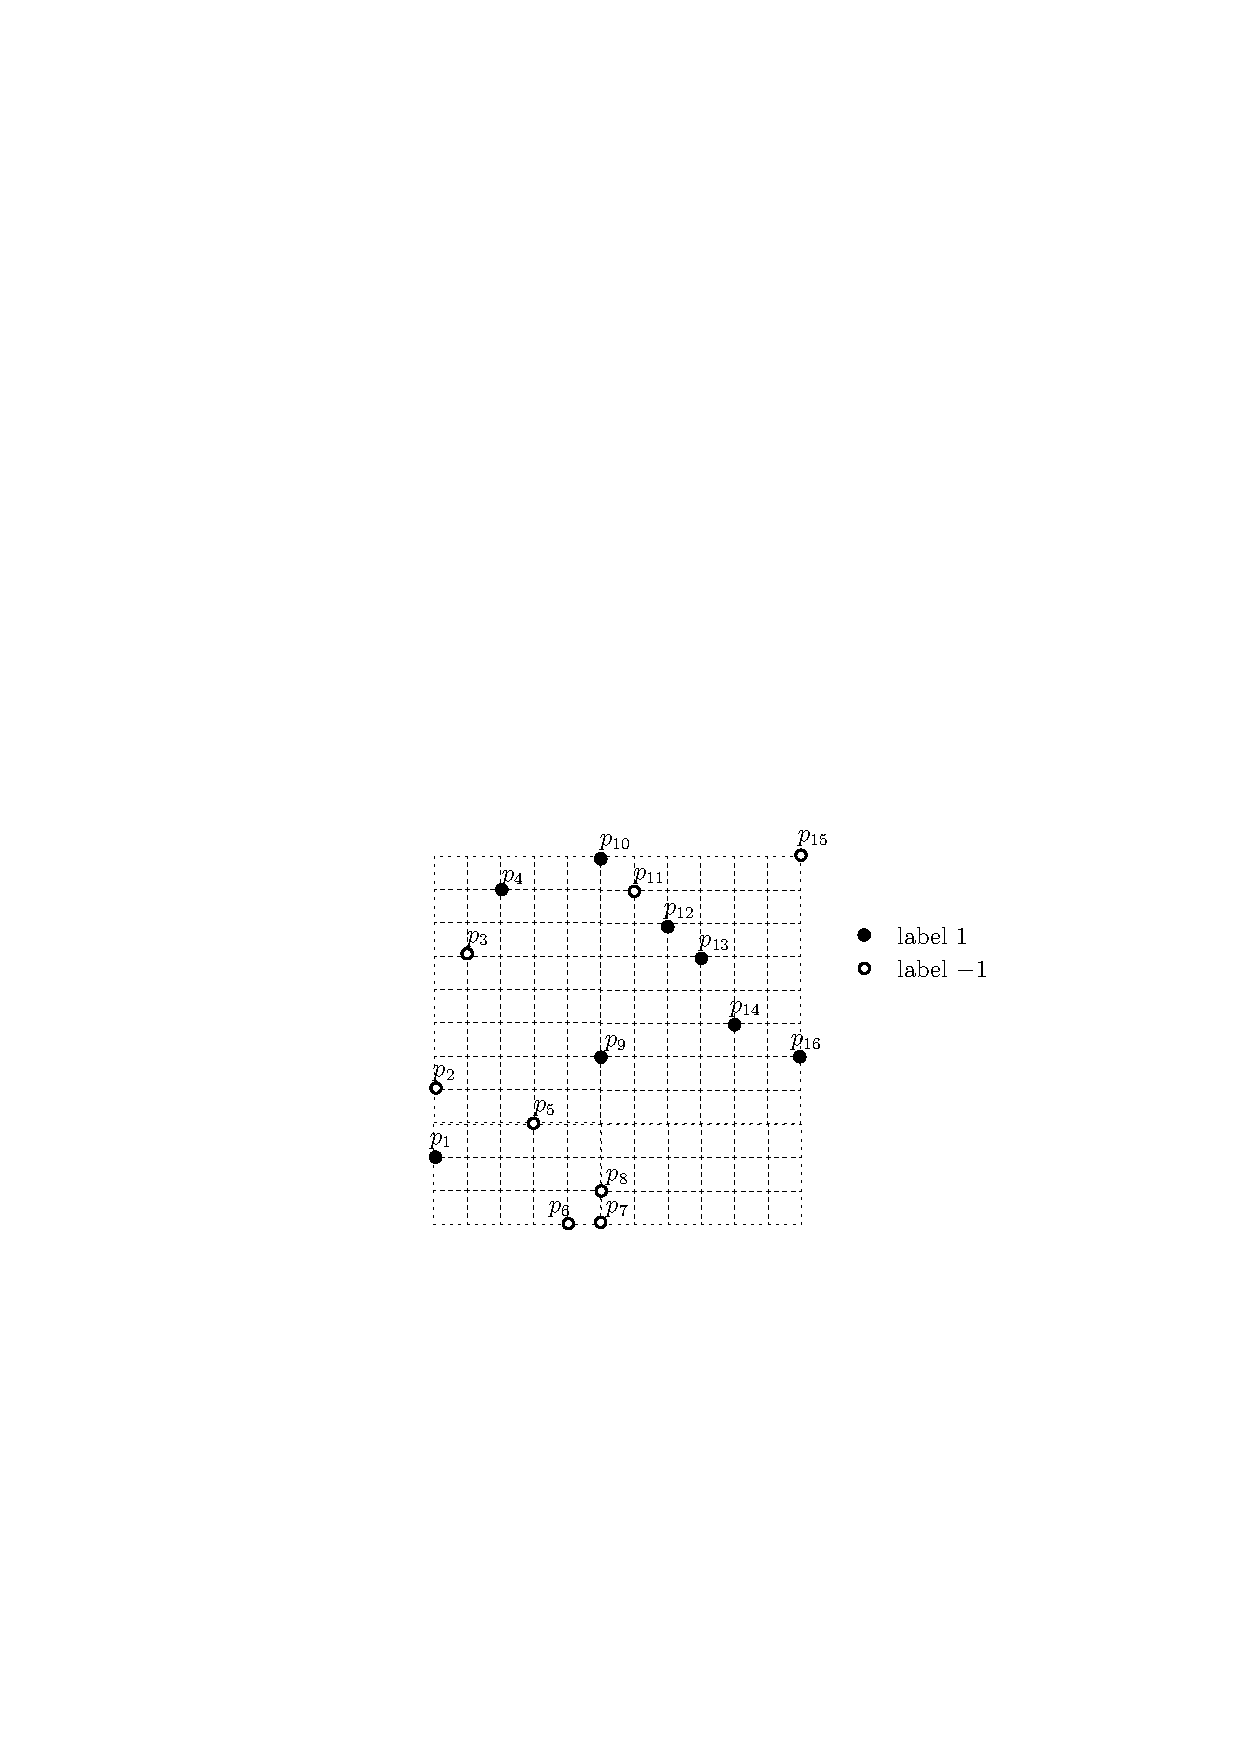
\includegraphics[height=55mm]{./artwork/ds}
    \figcapup
    \caption{An input set $P$ for Problem 1} \label{fig:intro-ds}
    \figcapdown
\end{figure}

\vgap

Toward the above purpose, a dominant methodology behind the existing approaches is to transform the task into a multidimensional classification problem with the following preprocessing.

\begin{enumerate}
    \item First, shrink the set of all possible pairs to a subset $S \subseteq E_1 \times E_2$, by eliminating pairs that clearly are not matches. This is known as {\em blocking}, which is carried out based on application-dependent heuristics. This step is optional; if skipped, then $S = E_1 \times E_2$. In the Amazon-eBay example, $S$ may involve only those advertisement pairs $(e_1, e_2)$ with $e_1.\ttt{year} = e_2.\ttt{year}$.

    \item For each entity pair $(e_1, e_2) \in S$, create a multidimensional point $p_{e_1, e_2}$ using several --- say $d$ --- similarity functions $\siml_1, \siml_2, ..., \siml_d$, each of which is evaluated on a certain attribute and produces a numeric ``feature''. The $i$-th coordinate of $p_{e_1,e_2}$ equals $\siml_i(e_1,e_2)$: a greater value indicates higher similarity between $e_1$ and $e_2$ under the $i$-th feature. This creates a $d$-dimensional point set $P = \{p_{e_1,e_2} \mid (e_1, e_2) \in S\}$. In our example, from a numerical attribute such as \ttt{price}, one may extract a similarity feature $-|e_1.\ttt{price} - e_2.\ttt{price}|$, where the negation is needed to ensure ``the larger the more similar''. From a text attribute (such as \ttt{prod-name} and \ttt{prod-description}) one may extract a similarity feature by evaluating the relevance between the corresponding texts of $e_1$ and $e_2$ using an appropriate metric (e.g., edit distance, jaccard-distance, cosine similarity, etc.). Multiple features may even be derived on the same attribute; e.g., one can extract two similarity features by computing the edit-distance and jaccard-distance of $e_1.\ttt{prod-name}$ and $e_2.\ttt{prod-name}$ separately.

    \item Every point $p_{e_1,e_2} \in P$ inherently carries a label, which is 1 if $(e_1,e_2)$ is a match, or $-1$ otherwise. The original entity matching task on $E_1$ and $E_2$ is now converted to inferring the labels of the points in $P$. Human inspection is the ultimate resort for determining the label of each $p_{e_1,e_2}$ with guaranteed correctness.
\end{enumerate}

%\vgap

Treating $P$ as the input for monotone classification, we can employ an algorithm $\A$ of monotone classification to significantly reduce human labor. Specifically, the human plays the role of oracle: when given a point $p_{e_1,e_2}$, the human ``reveals'' the label of $p_{e_1,e_2}$ by manually checking whether $e_1$ and $e_2$ are about the same entity. After a  number of probes (to the human oracle), the algorithm $\A$ outputs a monotone classifier $h \in \mono$, which is then used to infer the labels of the un-probed points in $P$. Demanding monotonicity is important for {\em explainable learning} because it avoids the odd situation of classifying $(e_1,e_2)$ as a non-match but $(e_1',e_2')$ as a match when $p_{e_1,e_2} \dom p_{e_1',e_2'}$. Indeed, this oddity is difficult to explain because the former pair is at least as similar as the latter on every feature.

\section{Remarks}

%\section{Remark} ksv10

\bibliographystyle{plainurl}% the mandatory bibstyle
\bibliography{ref}


\end{document}
